\subsection{Section 1 - About Me}

From Week 1, the definition of research is “a combination of investigation.” I hope to learn everything that I can about “investigation” and common tools in accomplishing that. I believe one of my skills, like reading research papers more effectively, can be further improved. More importantly, I bring in the mentality of being curious and grit. Being curious allows me to explore and wonder while grit allows me to dig deep into certain topics that would help with my research. My mission and goal for this CS6000 course is to get the perspective in understanding elements of good research that sparks my interest and passion, while making an impact on society. I am currently in my first semester of the PhD security program here at University of Colorado, Colorado Springs. With the nature of the program, I would also like to learn on how to effectively present my ideas and convey my research to the languages of different audiences. My research topic will be close to Blockchain technology with its performances and implementation. 

\begin{center}
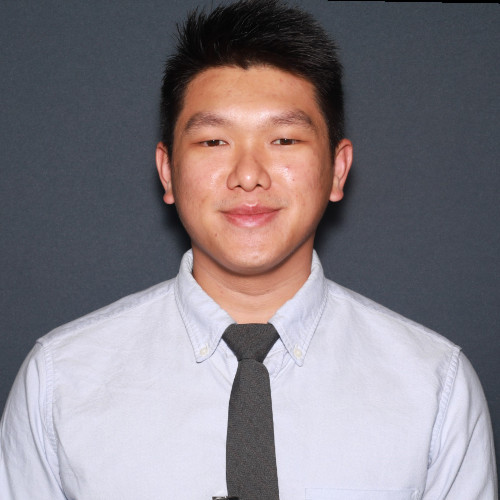
\includegraphics[scale=0.45]{kl.png}
\end{center}

Some of my recent interests besides information technology would be aviation and endurance sports. I have a little more than 100 hours in a Cessna 172M model and I will be running a 50k trail run this coming October.

\subsection{Section 2 - Git Repo}

\subsubsection{Git Repo - Research}
I found this Git Repo to be useful in learning more about Blockchain. This git repo covers topic from basics of blockchain all the way to development and implementation of blockchain.
\url{https://github.com/yjjnls/awesome-blockchain}


\subsubsection{Questions and Answer} 
You may include your question here:

\begin{enumerate}
    \item WW: Do you have anything interesting to share from your research into Blockchain thus far?
    \item Answer: I am looking into some high level material regarding Vehicle to Vehicle (V2V) process and the implementation of Blockchain in that area of technology.
    \item DH: Where are you doing your trail run, and is it with an organized team or an individual effort?
    \item Answer: I will be doing my 50k trail run at Palmer Park end of October. It is an organized event but yes, individual effort. Maybe in the future I will be brainstorming some races to include fund raising.
\end{enumerate}
